\documentclass[a4paper,11pt]{report}
\usepackage[T1]{fontenc}
\usepackage[utf8]{inputenc}
\usepackage[polish]{babel}
\usepackage{lmodern}
\usepackage{graphicx}

\title{czas obsługi: stosu, listy}
\author{Tomasz Piotrowski 200524}

\begin{document}
\maketitle

\textbf {\Large{ Sprawozdanie z czasu działania algorytmów  obsługi stosu oraz listy. }}



\begin{figure}
  \begin{center}
  1. Stos zrealizowany na tablicy. Rozmiar tablicy zwiekszany jesto o 1 w momencie dodawanie zmiennej. Oraz zmniejszany o 1 w momencie pobierania zmiennej. Na podstawie wykresu mżna stwierdzić że czas narasta logarytmicznie. 
    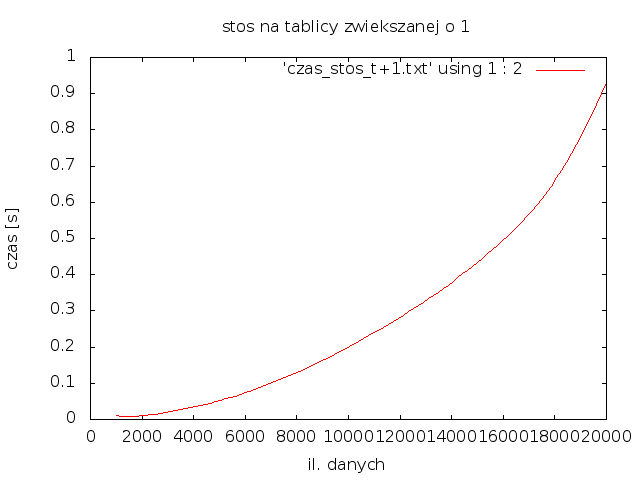
\includegraphics[scale=0.5]{./czas_stos_t+1.png}
    \label{fig:}
    \caption{}
  \end{center}
\end{figure}

\begin{figure}
  \begin{center}
  2. Stos zrealizowany na tablicy. Rozmiar tablicy zostaje zwiekszony dwukrotnie w momencie przepełnienia stosu. Rozmiar stosu zostaje zmniejszony dwukrotnie w momencie gdy jest zajmowany w 1/4 objetosci. Czas narasta proporcjonalie do ilosci danych.
    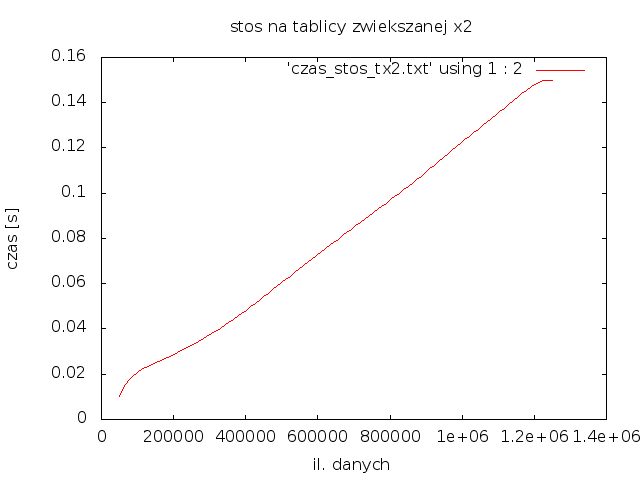
\includegraphics[scale=0.5]{./czas_stos_tx2.png}
    \label{fig:}
    \caption{}
  \end{center}
\end{figure}

\begin{figure}
  \begin{center}
  3. Stos zrealizowany za pomocą listy. W momencie dodawania nowej zmiennej tworzony jest nowy element. W odróżenienu od zwiększania tablicy o 1 w tym przypadku nie ma potrzeby wykonywania kopiowania czałego czasu. Czas wykonywania operacji na stosie wzrasta proporcjonalnie do ilości danych.
    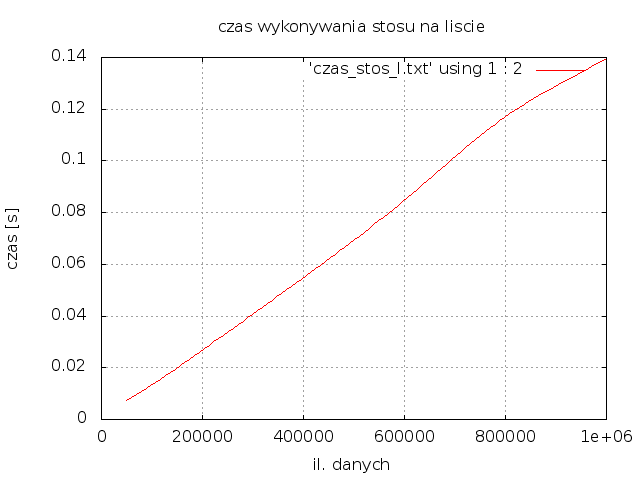
\includegraphics[scale=0.5]{./czas_stos_l.png}
    \label{fig:}
    \caption{}
  \end{center}
\end{figure}

\begin{figure}
  \begin{center}
  4. kolejka wykonana na liście. Czas obsługi proporcjnalny do ilości danych.
    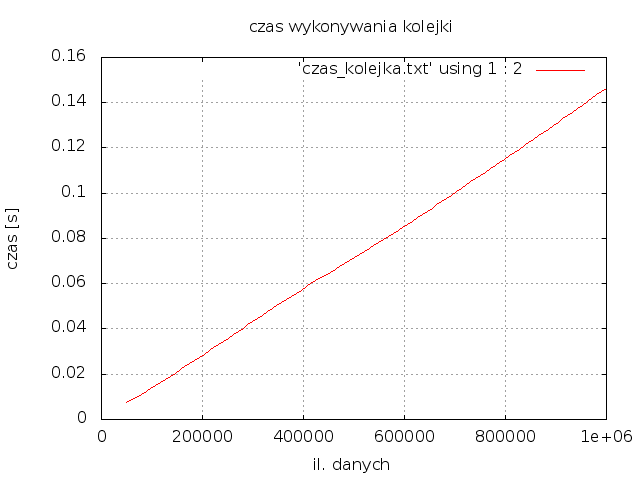
\includegraphics[scale=0.5]{./czas_kolejka.png}
    \label{fig:}
    \caption{}
  \end{center}
\end{figure}



\end{document}